\documentclass[14pt, russian, onesize]{extreport}

% BASE
\usepackage[a4paper, margin=0.5in]{geometry}
\usepackage{dingbat} % NICE LINEBREAK
\usepackage{graphicx}
\usepackage{amsmath}
\usepackage{amssymb}
\usepackage{enumitem}
\usepackage{amsfonts}
\usepackage{extarrows}
\usepackage{import}
\usepackage{indentfirst}
\usepackage{caption}
\captionsetup{justification=raggedright,singlelinecheck=false}
\usepackage{subcaption}
\usepackage{hyperref}
\usepackage{indentfirst}
\usepackage{color}
\usepackage{minted}
\usepackage{enumitem}

% FONTS XeLaTeX
\usepackage[no-math]{fontspec}
\usepackage{mathspec}
\defaultfontfeatures{Ligatures={TeX},Renderer=Basic}
\setmathfont(Digits){Times New Roman}
\setmainfont{Times New Roman}
\setsansfont{Arial}
\setmonofont{Consolas}
\newfontfamily\cyrillicfont[Script=Cyrillic]{Times New Roman}
\newfontfamily\cyrillicfontsf[Script=Cyrillic]{Arial}
\newfontfamily\cyrillicfonttt[Script=Cyrillic]{Consolas}
\usepackage{polyglossia}
\setdefaultlanguage{russian}

% MACRO
\delimitershortfall-1sp
\newcommand\abs[1]{\left|#1\right|}

% LISTINGS
\definecolor{bg}{rgb}{1,1,1}
\newminted{cpp}{linenos,fontsize=\footnotesize, bgcolor=bg, breakafter=, breaklines, breakautoindent=true, breaksymbolleft=\raisebox{0.8ex}{ \small\reflectbox{\carriagereturn}}, breaksymbolright=\small\carriagereturn, }
\newmintedfile{cpp}{fontsize=\footnotesize, bgcolor=bg, breaklines, breakafter=,}
\newenvironment{code}{\captionsetup{type=listing}}{}

% BASH
\usepackage{xparse}
\usepackage{etoolbox}
\usepackage{array}

\ExplSyntaxOn
\NewDocumentCommand{\captureshell}{som}
 {
  \sdaau_captureshell:Ne \l__sdaau_captureshell_out_tl { #3 }
  \IfBooleanT { #1 }
   {% we may need to stringify the result
    \tl_set:Nx \l__sdaau_captureshell_out_tl
     { \tl_to_str:N \l__sdaau_captureshell_out_tl }
   }
  \IfNoValueTF { #2 }
   {
    \tl_use:N \l__sdaau_captureshell_out_tl
   }
   {
    \tl_set_eq:NN #2 \l__sdaau_captureshell_out_tl
   }
 }

\tl_new:N \l__sdaau_captureshell_out_tl

\cs_new_protected:Nn \sdaau_captureshell:Nn
 {
  \sys_get_shell:nnN { #2 } { } #1
  \tl_trim_spaces:N #1 % remove leading and trailing spaces
 }
\cs_generate_variant:Nn \sdaau_captureshell:Nn { Ne }
\ExplSyntaxOff

\newcommand\ProcessOutput[1]{%
  \renewcommand*{\do}[1]{
      \begin{code}
          \caption{\textbf{##1}}
          \cppfile{##1}
      \end{code}
  }%
  \expandafter\docsvlist\expandafter{#1}%
}
\parindent=0pt

\makeatletter
\def\inputAllFiles#1#2{%
    \captureshell*[\cppfiles]{ls #1/*.#2 | paste -sd , -} 
    \ProcessOutput\cppfiles
}
\makeatother

% HYPERLINKS
\hypersetup{
    colorlinks=true,
    linkcolor=blue,
    filecolor=magenta,      
    urlcolor=blue,
}

% GRAPHICS
\usepackage{pgfplots}
\pgfplotsset{compat=1.9}
\graphicspath{ {../test_data} }


% START
\begin{document}
\begin{tabular}{|p{8cm}|p{3cm}|p{3cm}|}
    \hline
    Лабораторная работа №4 & Б10 & 2022\\
    \hline
    OpenMP  & \multicolumn{2}{|c|}{Хорохорин Андрей Сергеевич}\\
    \hline
\end{tabular}
\subsection*{ Цель работы }
Знакомство с основами многопоточного программирования.
\subsection*{ Инструментарий }
Секция генерируется автоматически при компиляции
\begin{enumerate}
    \item \captureshell{clang++ --version | head -n 1}
    \item \captureshell{vim --version | head -n 1}
    \item \captureshell{make --version | head -n 1}
    \item \captureshell{xelatex --version | head -n 1}
    \item OpenMP standard 2.0
\end{enumerate}

\section*{Описание конструкция OpenMP для распараллеливания команд}
В рамках работы мною были использованы следующие директивы OpenMP:
\begin{itemize}
    \item \texttt{\#pragma omp parallel}\\
        Объявляет начало блока, в котором код будет исполняться параллельно.
        Весь код вне этой директивы исполняется одним главным потоком. 
    \item \texttt{\#pragma omp for schedule(type, chunk)}\\
        Явно задаёт способ выполнения цикла на нескольких потоках. А именно
        каждая итерация объявляется как задача, а затем эти задачи распределяются
        по потокам. Само распределение может быть реализовано различным образом:
        за это отвечают аргументы type и chunk. Более подробно про различные
        распределения и их эффективность в данной задаче можно ознакомиться
        в \hyperref[experiment]{анализе результатов эксперимента}.
    \item \texttt{\#pragma omp critical}\\
        Объявляет некоторый блок кода как критическую секцию, также называемую
        mutex. Данная секция в каждый момент времени может исполняться лишь 
        одним потоком.
    \item \texttt{\#pragma omp threadprivate(variables)}
        По умолчанию все переменные объявленный внутри \texttt{omp parallel}
        являются локальными для потока, а все объявленные вне её: за 
        глобальные. Данная директива позволяет сделать исключение для 
        некоторого списка переменных, которые будут объявлены вне 
        \texttt{omp parallel}, но будут созданными для каждого
        из потоков в отдельности.
\end{itemize}
Помимо директив используются следующие runtime функции библиотеки:
\begin{itemize}
    \item \texttt{omp\_get\_wtime()}\\
        Возвращает астрономическое время, прошедшее после запуска
        программы. 
    \item \texttt{omp\_set\_num\_threads(n)}\\
        Устанавливает количество потоков по умолчанию, которые будут
        использованы для параллельного исполнения параллельных секций OpenMP.
\end{itemize}
\section*{Описание работы написанного кода}
Глобально можно поделить программу на 2 логические части. Первая из них это 
работа с изображением, включающее его ввод\slash вывод и трансформацию,
принимающую функцию, которая будет применена ко всем пикселям изображения.
Всё перечисленное реализовано в классе \texttt{PgmImage}. Думаю, не стоит отдельно
останавливаться на реализации данного класса, так как ничего интересного в ней
нет.

Вторая часть это сам алгоритм Оцу, определяющий по гистограмме цветов пороговые 
значения. Он реализован дважды: с директивами openmp и без. 

\textit{
Ps. Можно было конечно
завернуть все обращения к функциям из openmp в ifdef, компилировать в make две
версии программы: с fopenmp и без, а затем запускать нужную из них(в случае
-1 в качестве первого аргумента бинарник без openmp, иначе с ним) при
помощи bash скрипта. Но перелопачивать github CI мне не хочется.
}

Общая идея алгоритма следующая: изначально насчитываются взвешенные и не
взвешенные префиксные суммы для гистограммы цветов: 
\texttt{hist\_prefix} и \texttt{w\_hist\_prefix} соответственно. Далее
рекурсивной процедурой \texttt{get\_partition} перебираются все
разбиения и в функции \texttt{relax\_ans} для текущего разбиения 
подсчитывается целевая функция и, если смогли улучшить свой прошлый ответ, то
обновляем его на текущий.

\subsection*{Предподсчёт}
Функция \texttt{OtsuMultithread} является точкой входа в реализацию алгоритма.
В ней насчитывается \texttt{hist\_prefix} и \texttt{w\_hist\_prefix}, начинается
параллельная секция и инициализируются массивы \texttt{cur\_part} для каждого
из потоков, так как благодаря директиве \texttt{\#pragma omp threadprivate(cur\_part)}
он является локальным для каждого из потоков. Это необходимо, так как
каждый из потоков перебирает своё подмножество разбиений и очевидно, что для
хранения текущего разбиения каждого потока должна быть своя память.

После описанных выше действий запускается функция \texttt{get\_partition},
осуществляющая перебор разбиений.

\begin{cppcode}
#pragma omp threadprivate(cur_part)
vector<uint8_t> OtsuMultithread(const vector<unsigned int>& hist) {
    N = std::accumulate(hist.begin(), hist.end(), 0);
    hist_prefix.resize(MAXP + 1, 0);
    w_hist_prefix.resize(MAXP + 1, 0);

    for (size_t i = 1; i <= MAXP; ++i) {
        hist_prefix[i] = hist_prefix[i - 1] + hist[i - 1];
        w_hist_prefix[i] = w_hist_prefix[i - 1] + 1ll * hist[i - 1] * (i - 1);
    }

#pragma omp parallel 
    {
        cur_part.resize(M - 1);
        get_partition(1, 0);
    }
    return part;
}
\end{cppcode}
\subsection*{Перебор разбиений} \label{implementation}
Реализация перебора является рекурсивной, благодаря чему работает для 
произвольного количества цветовых зон, на которые делится изображение.

Важной деталью реализации тут является то, что распараллеливается только цикл
перебирающий первую границу разбиения. 
В противном случае слишком много маленьких итераций, что работает на порядок 
медленнее, чем данное решение. 

Отметим то, что итерации в моей реализации имеют
различную вычислительную сложность, так как чем меньше первая граница,
тем больше существует разбиений оставшейся части цветов. Эта деталь во многом
определяет выбор оптимального параметра для \texttt{schedule}.

\begin{cppcode}
void get_partition(int tl, int cur_th) {
    if (cur_th == M - 1) {
        relax_ans();
    } else if (cur_th == 0) {
#pragma omp for schedule(dynamic, 1)
        for (size_t i = tl; i < MAXP; ++i) {
            cur_part[cur_th] = i;
            get_partition(i + 1, cur_th + 1);
        }
    } else {
        for (size_t i = tl; i < MAXP; ++i) {
            cur_part[cur_th] = i;
            get_partition(i + 1, cur_th + 1);
        }
    }
}
\end{cppcode}
\subsection*{Обновление ответа}
В функции \texttt{relax\_ans}, насчитывается значение целевой функции для
текущего разбиения на слагаемые, пользуясь подсчитанными 
\texttt{hist\_prefix} и \texttt{w\_hist\_prefix}. Отдельно стоит отметить,
что в данной функции есть запись в общие для потоков ячейки памяти 
\texttt{part} и \texttt{part\_disp} и если два потока захотят одновременно
обновить в них значения получится не пойми что, поэтому необходимо сделать обновление 
ответа в критической секцией.

Помимо этого, просто глядя на код не понятно, почему на строчках 19-27
написан такой велосипед. Почему же нельзя было просто обойтись одним if 
внутри критической секции? Потому что в таком случае это условие являлось
бы бутылочным горлышком нашего алгоритма: потоки постоянно ждали бы доступа
к проверке того, что их текущий ответ хуже, чем уже найденный, что происходит
почти всегда. Такая реализация будет работать гораздо хуже даже однопоточной.
\begin{cppcode}
// [tl, tr)
std::pair<unsigned long long, double> get_sums_for_part(int tl, int tr) {
    unsigned long long q = get_sum(hist_prefix, tl, tr);
    double mu = 1.0 * get_sum(w_hist_prefix, tl, tr) / q;
    return {q, mu};
}

void relax_ans() {
    double cur_disp = 0;
    auto [q, mu] = get_sums_for_part(0, cur_part.front());
    cur_disp += q * mu * mu;
    for (size_t i = 1; i < cur_part.size(); ++i) {
        std::tie(q, mu) = get_sums_for_part(cur_part[i - 1], cur_part[i]);
        cur_disp += q * mu * mu;
    }
    std::tie(q, mu) = get_sums_for_part(cur_part.back(), MAXP);
    cur_disp += q * mu * mu;

    if (cur_disp > part_disp) {
#pragma omp critical
        {
            if (cur_disp > part_disp) {
                part = cur_part;
                part_disp = cur_disp;
            }
        }
    }
}
\end{cppcode}
\section*{Результат работы программы}
Секция генерируется автоматически при компиляции

Модель процессора, на котором проводилось тестирование:

\texttt{ \captureshell*{cat /proc/cpuinfo | grep 'model name' | head -n 1} }

\texttt{ \captureshell*{make -sC ../ single} }

\def\inputverbatim #1{\bgroup
  \def\do##1{\catcode`##1=12 }\dospecials
  \def\par{\endgraf\noindent\null}\obeylines\obeyspaces
  \tt \noindent
    \input{#1}
  \egroup
}

\captureshell*[\devnull]{convert ../out.pgm ../out/png &> /dev/null} 

\begin{figure}[H]
    \centering
    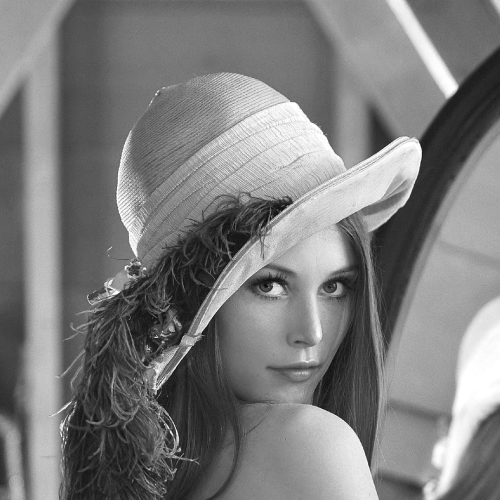
\includegraphics[width=0.45\textwidth]{in.png}
    \quad
    \includegraphics[width=0.45\textwidth]{../out.png}
\end{figure}

\section*{Экспериментальная часть}\label{experiment}
Все результаты по времени, изображённые на графиках ниже, взяты как 
сумма времени исполнения 10 последовательных запусков. Замеры
производились следующим скриптом, использовалась директива \texttt{schedule(runtime)}
для управления schedule через переменную окружения.
\inputminted[fontsize=\footnotesize]{bash}{../runner.sh}

\begin{tikzpicture}
    \begin{axis}[
        title = Стандартные chunk\_size,
        xlabel = {потоки},
        xtick={1,2,3,4},
        xmin = 0,
        ylabel = {время, ms},
        legend pos = north east
        ]
        \legend{ 
            dynamic, 
            static,
            guided,
        };
        \addplot[blue, mark = *] table {
            th time
            1  1.317469
            2  0.7849083
            3  0.5440092
            4  0.4044590
        };
        \addplot[red, mark = *] table {
            th time
          1 1.310493
          2 1.108694
          3 1.0002051
          4 1.0508911
        };
        \addplot[green, mark = *] table {
            th time
         1 1.510582
         2 .9630511
         3 .7189546
         4 .5656959
        };
        \addplot[dashed, draw = black] {0.8622980};
    \end{axis}
\end{tikzpicture}
\begin{tikzpicture}
    \begin{semilogxaxis}[
        log basis x=2,
        title = Различные chunk\_size на 4-х потоках,
        xlabel = {chunk\_size},
        xtick  = {1, 2, 4, 8, 16, 32, 64},
        ylabel = {время, ms},
        legend pos = north west
        ]
        \legend{ 
            dynamic, 
            static,
            guided,
        };
        \addplot[blue, mark = *] table {
            th time
            1 .4295223
            2 .4336456
            4 .4312994
            8 .4928696
           16 .9589350
           32 .8740137
           64 .9642729
        };
        \addplot[red, mark = *] table {
            1 .4704731
            2 .4771130
            4 .5105021
            8 .5519331
           16 .5769851
           32 .7102234
           64 1.0508911
        };
        \addplot[green, mark = *] table {
            th time
            1 .5656959
            2 .5761520
            4 .5677764
            8 .6263544
           16 .7070798
           32 .7851832
           64 1.176031
        };
        \addplot[dashed, domain = 0:64, draw = black] table {
            th time
            1 0.8622980
           64 0.8622980
        };
    \end{semilogxaxis}
\end{tikzpicture}

Пунктирной линией показано время работы программы на одном потоке без OpenMP.
На самом деле в данной ситуации какое-то время тратится на инициализацию OpenMP,
даже если код не заходит в параллельную секцию, поэтому можно думать, что
реальное время работы одного пока немного меньше.

Давайте я вкратце расскажу про различные schedule и поймём, почему результаты
именно такие.
\begin{itemize}
    \item \texttt{dynamic}~--- создаёт очередь из всех задач, после того,
        как поток освободился мы отдаём ему очередную задачу на исполнение.
    \item \texttt{static}~--- для каждого из потоков задачи распределены
        заранее примерно поровну. Но вот на сколько это поровну окажется близким
        к правде может сильно варьироваться.
    \item \texttt{guided}~--- работает похожим на dynamic образом, но планировщик
        пытается составить очередь с уменьшением размера исполняемой задачи.
        Теоретически это хорошо, потому что не может получиться так,
        что в конце одному из потоков достанется большая задача, которую он
        будет исполнять, когда как другие потоки будут просто простаивать.
\end{itemize}
Могу предположить, что \texttt{guided} работает медленнее \texttt{dynamic},
так как планировщику требуется дополнительно много времени на планирование и не 
факт что оно будет успешным, а размер итераций в моей реализации всегда убывает
просто как следствие \hyperref[implementation]{структуры алгоритма}. 
\texttt{static} хорошо подходит для ситуаций, когда потоков очень много и
\texttt{dynamic} тратит много времени на реализацию очереди задач. Но у меня
ядер мало, поэтому \texttt{static} показывает себя не очень хорошо.

\section*{Список источников}
\begin{itemize}
    \item \href{https://www.openmp.org//wp-content/uploads/cspec20.pdf}
        {Документация по OpenMP}
\end{itemize}

\section*{Листинг кода}
Секция генерируется автоматически при компиляции
\inputAllFiles{../include}{h}

\inputAllFiles{../src}{cpp}


\end{document}
